\documentclass[aspectratio=169,10pt]{beamer}

\usepackage[utf8]{inputenc}
\usepackage[T1]{fontenc}
\usepackage[spanish,es-nodecimaldot]{babel}
\usepackage{booktabs}
\usepackage{array}
\usepackage{graphicx}
\usepackage{amssymb}
\usepackage{tikz}
\usetikzlibrary{arrows.meta,positioning,shapes.geometric,fit}

\definecolor{navy}{HTML}{173F5F}
\definecolor{teal}{HTML}{2A9D8F}
\definecolor{orange}{HTML}{F4A261}
\definecolor{coral}{HTML}{E76F51}
\definecolor{slate}{HTML}{475569}
\definecolor{mist}{HTML}{EEF4F7}
\definecolor{cream}{HTML}{FFF5EB}

\setbeamercolor{normal text}{fg=slate,bg=white}
\setbeamercolor{structure}{fg=navy}
\setbeamercolor{frametitle}{fg=navy,bg=white}
\setbeamercolor{title}{fg=navy}
\setbeamercolor{subtitle}{fg=teal}
\setbeamercolor{block title}{fg=white,bg=navy}
\setbeamercolor{block body}{fg=slate,bg=mist}
\setbeamercolor{alerted text}{fg=coral}
\setbeamerfont{title}{series=\bfseries,size=\LARGE}
\setbeamerfont{frametitle}{series=\bfseries,size=\Large}
\setbeamerfont{subtitle}{size=\large}
\setbeamertemplate{navigation symbols}{}
\setbeamertemplate{itemize item}{\color{teal}$\blacktriangleright$}
\setbeamertemplate{itemize subitem}{\color{orange}$\bullet$}
\setbeamertemplate{footline}{%
  \leavevmode\hbox{%
    \begin{beamercolorbox}[wd=.82\paperwidth,ht=2.6ex,dp=1.1ex,leftskip=1em]{author in head/foot}%
      \color{slate}\scriptsize INFO1185 · Detección de fraude
    \end{beamercolorbox}%
    \begin{beamercolorbox}[wd=.18\paperwidth,ht=2.6ex,dp=1.1ex,rightskip=1em plus1fil]{date in head/foot}%
      \color{navy}\scriptsize\insertframenumber
    \end{beamercolorbox}}%
}
\setbeamertemplate{headline}{\vspace{0.25em}}
\setbeamersize{text margin left=0.65cm,text margin right=0.65cm}

\graphicspath{{figures/}}
\newcommand{\good}[1]{\textcolor{teal}{\textbf{#1}}}
\newcommand{\warn}[1]{\textcolor{coral}{\textbf{#1}}}
\newcommand{\muted}[1]{\textcolor{slate}{#1}}
\newcommand{\ros}{\textbf{ROS}}

\title{Detección de fraude con aprendizaje supervisado}
\subtitle{Minimizar fraudes no detectados sin ignorar las falsas alarmas}
\author{Máximo Mora \and Diego Álvarez}
\institute{INFO1185 — Inteligencia Artificial}
\date{Octubre de 2026}

\begin{document}

% 1
\begin{frame}[plain]
  \titlepage
  \vspace{-1.3em}
  \begin{center}
    \begin{beamercolorbox}[wd=.88\textwidth,rounded=true,sep=.65em,center]{block body}
      \large Objetivo: detectar transacciones fraudulentas priorizando la
      \warn{minimización de falsos negativos (FNR)}.
    \end{beamercolorbox}
  \end{center}
\end{frame}

% 2
\begin{frame}{1. Datos: el fraude es excepcional}
  \begin{columns}[T,onlytextwidth]
    \column{.53\textwidth}
      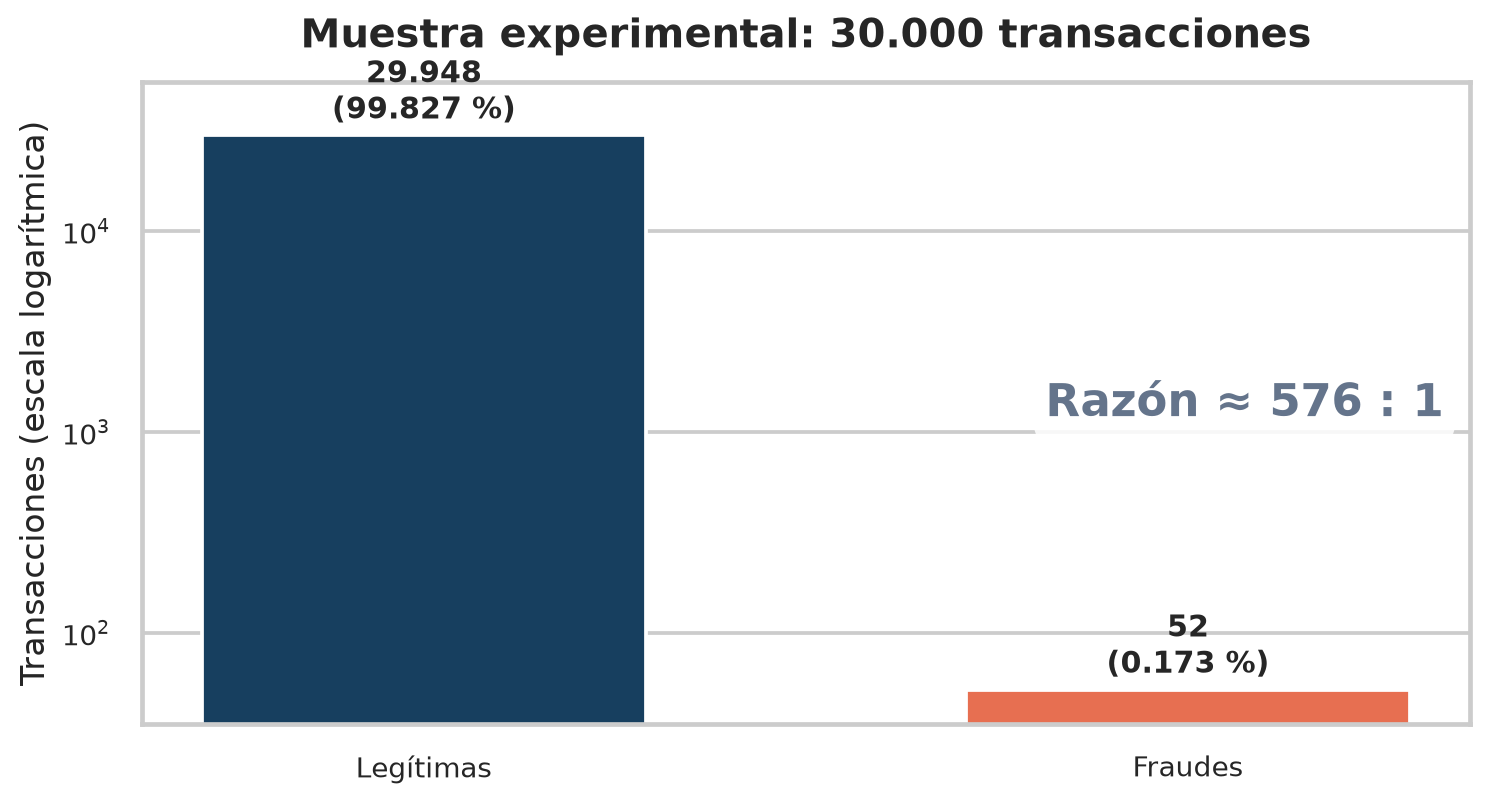
\includegraphics[width=\linewidth]{class_distribution.png}
    \column{.44\textwidth}
      \vspace{0.3em}
      \begin{block}{Credit Card Fraud Detection}
        \begin{itemize}\setlength\itemsep{.45em}
          \item Fuente: 284.807 registros; experimento: \textbf{30.000}.
          \item 30 predictores: \texttt{Time}, \texttt{Amount}, \texttt{V1--V28}.
          \item Objetivo: \texttt{Class}; fraude = clase positiva.
          \item 29.948 legítimas y 52 fraudes (0,173\%).
        \end{itemize}
      \end{block}
      \small
      Sin valores faltantes. Los 1.081 duplicados del dataset fuente se
      conservaron, pero se agruparon al dividir para evitar copias cruzadas.
  \end{columns}
\end{frame}

% 3
\begin{frame}{2. Metodología sin fuga de información}
  \centering
  \resizebox{\linewidth}{!}{%
  \begin{tikzpicture}[
    node distance=5mm and 5mm,
    every node/.style={font=\scriptsize,align=center},
    box/.style={rounded corners=2pt,draw=navy,very thick,fill=mist,minimum height=11mm,text width=25mm},
    train/.style={box,fill=teal!12,draw=teal},
    test/.style={box,fill=orange!18,draw=orange},
    arrow/.style={-{Latex[length=2mm]},thick,draw=slate}
  ]
    \node[box] (sample) {Muestra estratificada\\30.000 · semilla 42};
    \node[train,right=of sample] (split) {División 70/30\\21.000 train};
    \node[train,right=of split] (folds) {CV estratificada\\5 folds compartidos};
    \node[train,right=of folds] (inside) {Por training fold\\escalar \(\rightarrow\) seleccionar 10\\\(\rightarrow\) \ros{} opcional \(\rightarrow\) entrenar};
    \node[train,right=of inside] (select) {Elegir por sensibilidad\\desempate: precisión};
    \node[test,below=8mm of select] (final) {Reentrenar con 70\%\\evaluar una vez en test};
    \node[test,left=of final] (holdout) {30\% reservado\\9.000 registros};
    \draw[arrow] (sample) -- (split);
    \draw[arrow] (split) -- (folds);
    \draw[arrow] (folds) -- (inside);
    \draw[arrow] (inside) -- (select);
    \draw[arrow] (select) -- (final);
    \draw[arrow] (split.south) |- (holdout.west);
    \draw[arrow] (holdout) -- (final);
  \end{tikzpicture}
  }

  \vspace{0.65em}
  \begin{columns}[T,onlytextwidth]
    \column{.48\textwidth}
      \begin{block}{Preprocesamiento}
        StandardScaler para k-NN/SVM; árboles sin escalado. SelectKBest por
        información mutua se ajusta dentro de cada fold.
      \end{block}
    \column{.48\textwidth}
      \begin{block}{Regla de aislamiento}
        Validación y test nunca se balancean ni participan en selección de
        variables, hiperparámetros o umbrales.
      \end{block}
  \end{columns}
\end{frame}

% 4
\begin{frame}{3. Cuatro clasificadores, cuatro sesgos inductivos}
  \begin{columns}[T,onlytextwidth]
    \column{.49\textwidth}
      \begin{block}{k-Nearest Neighbors}
        Vota entre vecinos según distancia. Es sensible a la escala y al valor
        de \(k\); se evaluaron distancias euclídea y Manhattan.
      \end{block}
      \begin{block}{Árbol de Decisión}
        Divide el espacio con reglas interpretables. Puede sobreajustar; se
        controlaron profundidad y tamaños mínimos de nodos.
      \end{block}
    \column{.49\textwidth}
      \begin{block}{Support Vector Machine}
        Busca una frontera con margen amplio. Requiere escalado; se compararon
        kernels lineal y RBF y distintos valores de \(C\).
      \end{block}
      \begin{block}{Random Forest propio}
        Combina árboles diversos mediante bootstrap, aleatoriedad de atributos
        y voto mayoritario para reducir varianza.
      \end{block}
  \end{columns}
\end{frame}

% 5
\begin{frame}{4. Random Forest propio: bootstrap + bagging}
  \begin{columns}[T,onlytextwidth]
    \column{.61\textwidth}
      \centering
      \resizebox{\linewidth}{!}{%
      \begin{tikzpicture}[
        node distance=5mm and 5mm,
        every node/.style={font=\scriptsize,align=center},
        data/.style={rounded corners,draw=navy,thick,fill=mist,minimum height=9mm,text width=24mm},
        tree/.style={circle,draw=teal,very thick,fill=teal!12,minimum size=12mm},
        vote/.style={rounded corners,draw=coral,very thick,fill=cream,minimum height=11mm,text width=24mm},
        arrow/.style={-{Latex[length=2mm]},thick,draw=slate}
      ]
        \node[data] (train) {Training disponible\\\(n\) filas};
        \node[data,right=8mm of train,yshift=14mm] (b1) {Bootstrap 1\\\(n\), con reemplazo};
        \node[data,right=8mm of train] (b2) {Bootstrap 2\\\(n\), con reemplazo};
        \node[data,right=8mm of train,yshift=-14mm] (bk) {Bootstrap \(B\)\\\(n\), con reemplazo};
        \node[tree,right=8mm of b1] (t1) {Árbol 1};
        \node[tree,right=8mm of b2] (t2) {Árbol 2};
        \node[tree,right=8mm of bk] (tk) {Árbol \(B\)};
        \node[vote,right=12mm of t2] (vote) {Voto mayoritario\\clase con más votos};
        \draw[arrow] (train) -- (b1);
        \draw[arrow] (train) -- (b2);
        \draw[arrow] (train) -- (bk);
        \draw[arrow] (b1) -- (t1);
        \draw[arrow] (b2) -- (t2);
        \draw[arrow] (bk) -- (tk);
        \draw[arrow] (t1) -- (vote);
        \draw[arrow] (t2) -- (vote);
        \draw[arrow] (tk) -- (vote);
      \end{tikzpicture}
      }
      \vspace{0.5em}

      \small Registros repetidos son esperables: cada sorteo se hace
      \textbf{con reemplazo}. Cada árbol aprende una vista distinta.
    \column{.36\textwidth}
      \begin{block}{Implementación real}
        \begin{itemize}\setlength\itemsep{.4em}
          \item \texttt{DecisionTreeClassifier} como base.
          \item \texttt{max\_features} aleatorio en cada división.
          \item Semillas únicas derivadas de la semilla 42.
          \item \texttt{n\_estimators}, \texttt{max\_depth},
                \texttt{max\_features} configurables.
          \item Búsqueda usa 5 u 11 árboles: siempre impar.
        \end{itemize}
      \end{block}
      \small No se usa \texttt{RandomForestClassifier} ni
      \texttt{BaggingClassifier}.
  \end{columns}
\end{frame}

% 6
\begin{frame}{5. Desbalance: ocho condiciones comparables}
  \begin{columns}[T,onlytextwidth]
    \column{.52\textwidth}
      \centering
      \renewcommand{\arraystretch}{1.18}
      \resizebox{\linewidth}{!}{%
      \begin{tabular}{lcc}
        \toprule
        Modelo & Sin compensación & Con \ros{} \\
        \midrule
        k-NN & \checkmark & \checkmark \\
        SVM & \checkmark & \checkmark \\
        Árbol & \checkmark & \checkmark \\
        Random Forest propio & \checkmark & \checkmark \\
        \bottomrule
      \end{tabular}
      }
      \vspace{1em}

      \begin{beamercolorbox}[wd=.92\linewidth,rounded=true,sep=.7em,center]{block body}
        Entrenamiento completo: \textbf{20.964 : 36}\\
        después de \ros{}: \textbf{20.964 : 20.964}
      \end{beamercolorbox}
    \column{.45\textwidth}
      \begin{block}{RandomOverSampler}
        Duplica fraudes elegidos al azar hasta igualar la clase mayoritaria. No
        inventa puntos sintéticos y conserva todos los ejemplos originales.
      \end{block}
      \begin{block}{Dónde se aplica}
        Solo al \textbf{training fold}, después de escalado/selección. En el
        Random Forest, cada bootstrap parte de ese training disponible.
      \end{block}
      \small
      Efecto esperado: más fraudes detectados, pero potencialmente más falsos
      positivos. El resultado debe comprobarse por modelo.
  \end{columns}
\end{frame}

% 7
\begin{frame}{6. Búsqueda y selección de hiperparámetros}
  \begin{columns}[T,onlytextwidth]
    \column{.57\textwidth}
      \small
      \renewcommand{\arraystretch}{1.17}
      \resizebox{\linewidth}{!}{%
      \begin{tabular}{>{\bfseries}p{.22\linewidth}p{.70\linewidth}}
        \toprule
        Modelo & Espacio acotado: cuatro candidatos \\
        \midrule
        k-NN & \(k\in\{3,5,7,11\}\); peso uniforme/distancia; euclídea/Manhattan \\
        SVM & kernel lineal/RBF; \(C\in\{0{,}5,2\}\); \(\gamma\) scale/0,1 \\
        Árbol & profundidad libre/12; split 2/20; hoja 1/5; gini/entropía \\
        RF propio & 5/11 árboles; profundidad libre/12; \(\sqrt{p}\)/\(\log_2p\) \\
        \bottomrule
      \end{tabular}
      }
      \vspace{0.8em}

      \begin{block}{Criterio común}
        Cinco folds compartidos. Maximizar \textbf{sensibilidad media}; ante
        empate, maximizar \textbf{precisión media}.
      \end{block}
    \column{.40\textwidth}
      \begin{beamercolorbox}[wd=\linewidth,rounded=true,sep=.8em]{block body}
        \centering
        \textbf{Configuración global seleccionada}\\[.45em]
        \Large SVM lineal + \ros{}\\[.35em]
        \normalsize \(C=0{,}5\)\\[.55em]
        Sensibilidad CV\\
        \good{0,9179 \(\pm\) 0,0674}\\[.25em]
        FNR CV: 0,0821 \(\pm\) 0,0674
      \end{beamercolorbox}
      \vspace{0.7em}
      \scriptsize
      Variables del ajuste final: V3, V4, V7, V10, V11, V12, V14, V16, V17 y V18.
  \end{columns}
\end{frame}

% 8
\begin{frame}{7. Validación cruzada: sensibilidad vs. precisión}
  \centering
  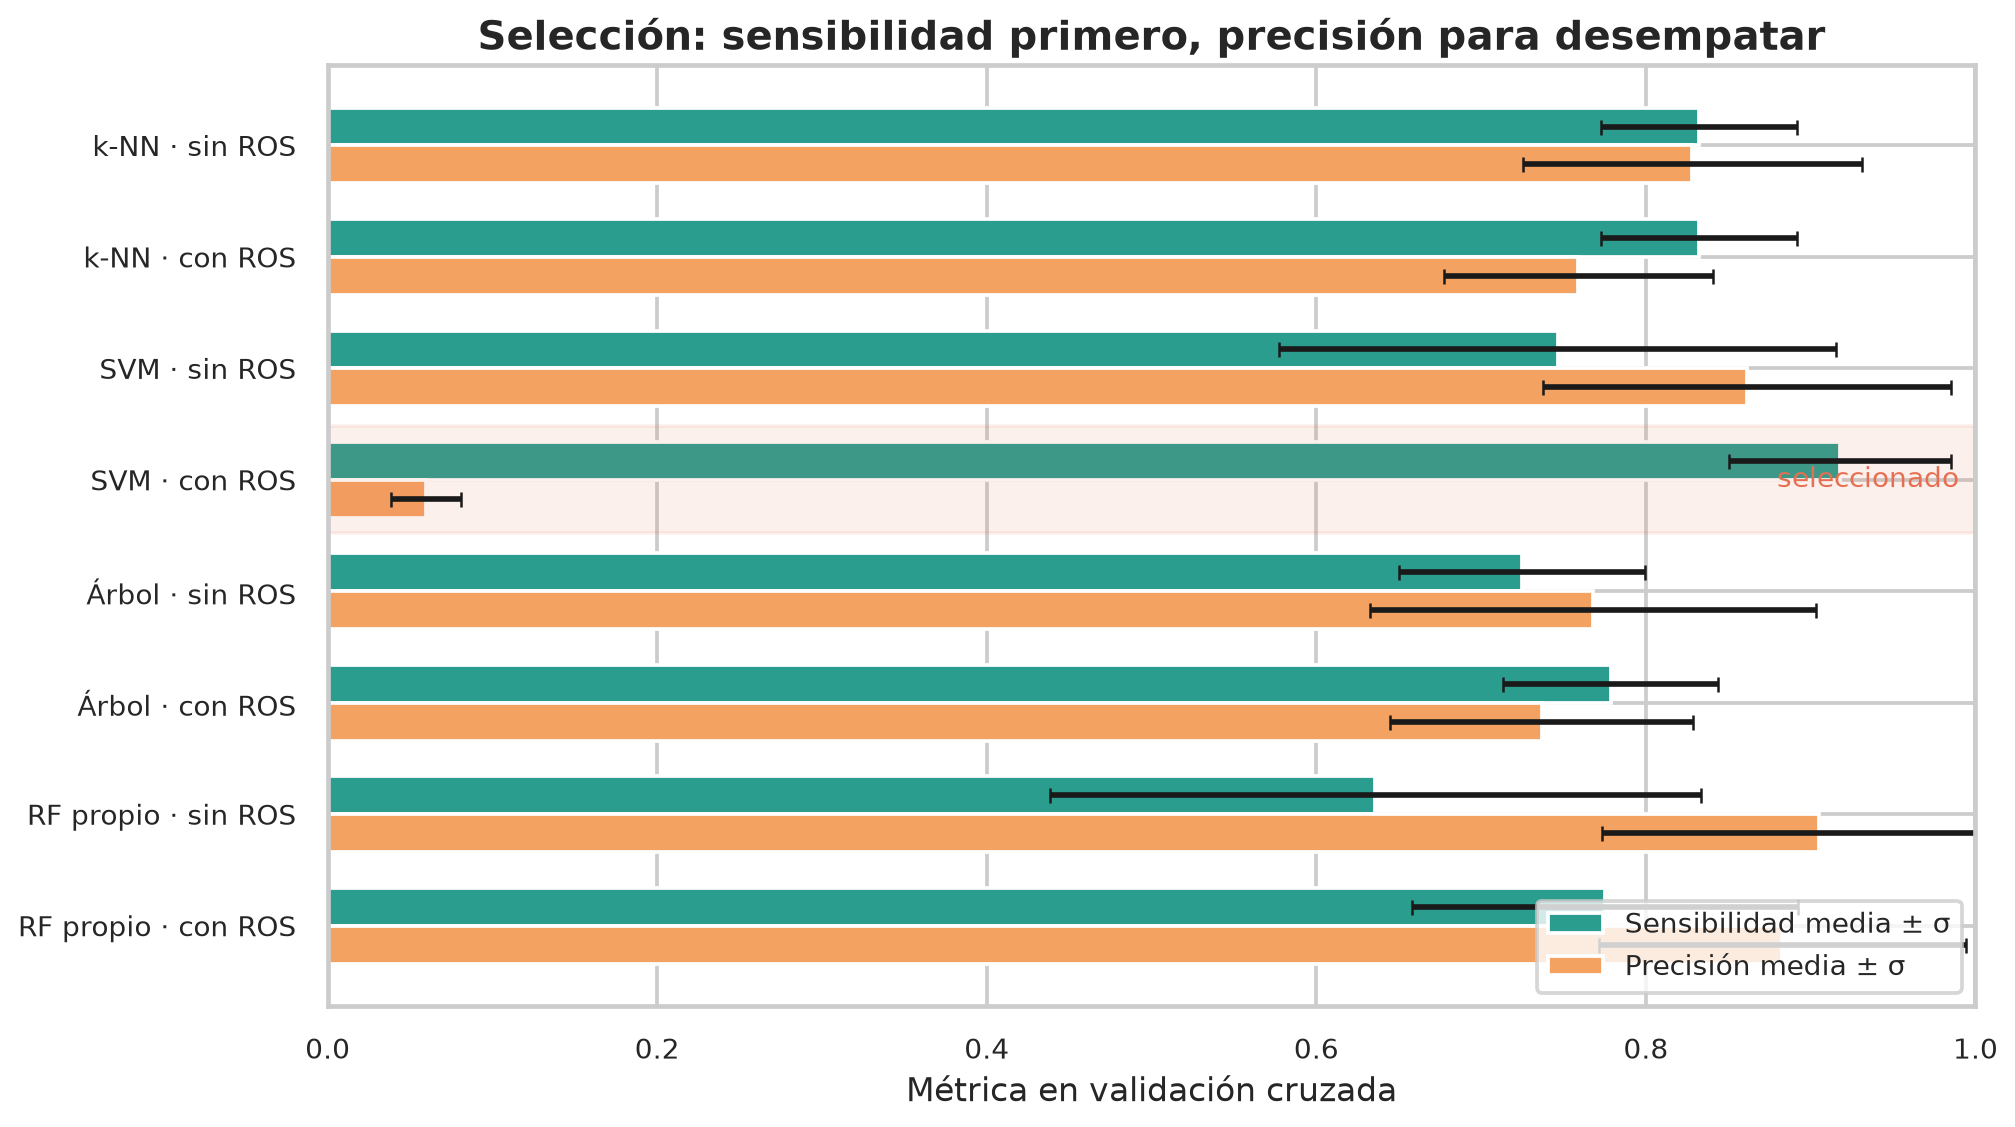
\includegraphics[height=.77\textheight]{cv_tradeoff.png}

  \vspace{-0.35em}
  \small La SVM balanceada domina en sensibilidad media, pero anticipa un costo:
  su precisión media es solo \warn{5,96\%}.
\end{frame}

% 9
\begin{frame}{8. Prueba reservada: resultado final de las ocho condiciones}
  \begin{columns}[T,onlytextwidth]
    \column{.66\textwidth}
      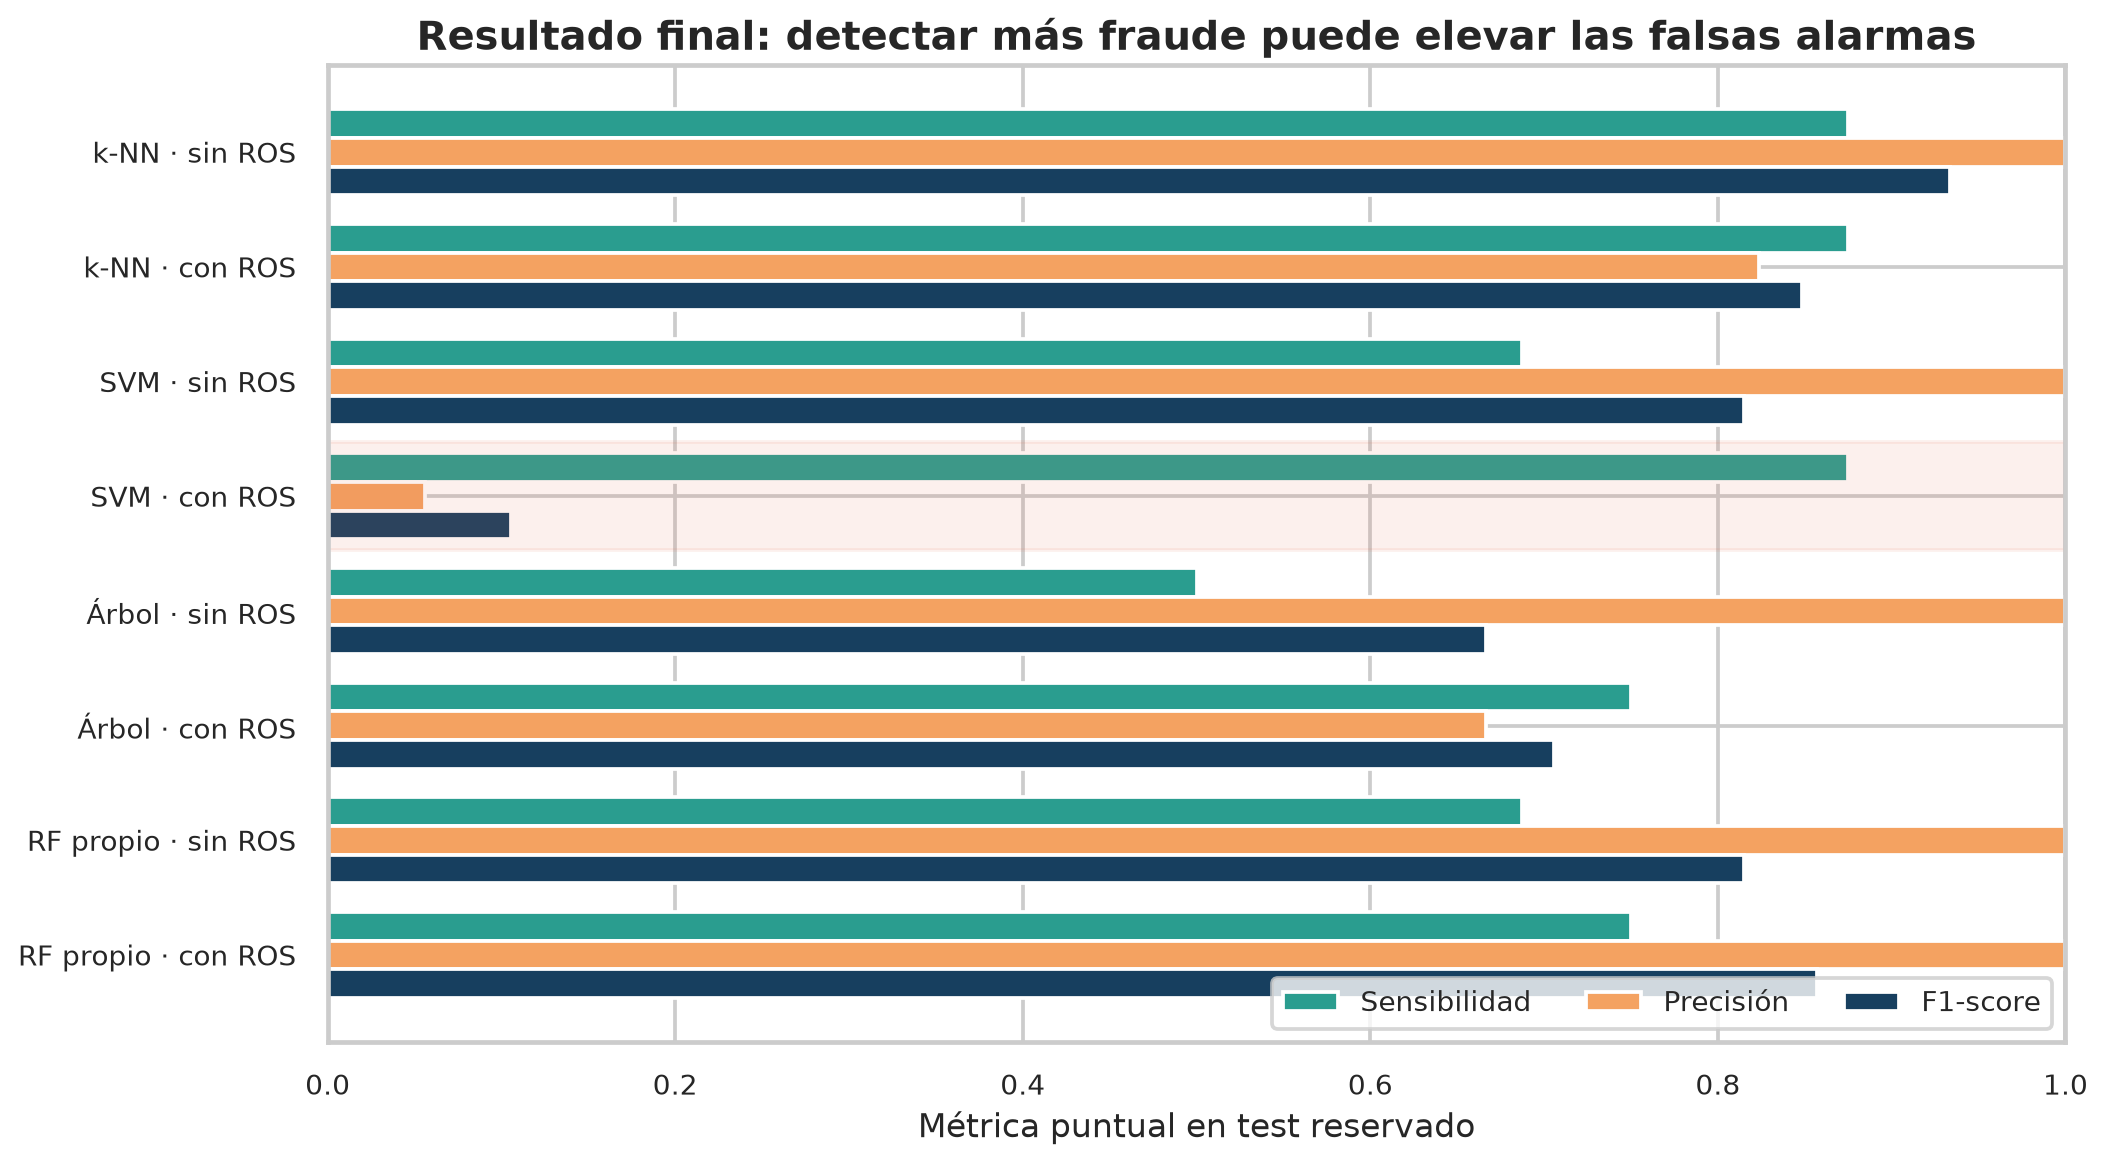
\includegraphics[width=\linewidth]{test_tradeoff.png}
    \column{.32\textwidth}
      \begin{beamercolorbox}[wd=\linewidth,rounded=true,sep=.65em]{block body}
        \centering\textbf{SVM + \ros{} en test}\\[.35em]
        \scriptsize
        \begin{tabular}{lr}
          Sensibilidad & 0,8750 \\
          Especificidad & 0,9738 \\
          Precisión & 0,0562 \\
          F1-score & 0,1057 \\
          Exactitud & 0,9737 \\
          FNR & 0,1250 \\
        \end{tabular}\\[.45em]
        \textbf{TN 8.749 · FP 235 · FN 2 · TP 14}
      \end{beamercolorbox}
      \vspace{.65em}
      \scriptsize
      Evaluación única sobre 9.000 casos. Las dispersiones reportadas en respaldo
      son bootstrap estratificado (200 remuestras) de predicciones fijas, no
      variación entre reentrenamientos.
  \end{columns}
\end{frame}

% 10
\begin{frame}{9. Análisis crítico: sensibilidad no basta}
  \begin{columns}[T,onlytextwidth]
    \column{.53\textwidth}
      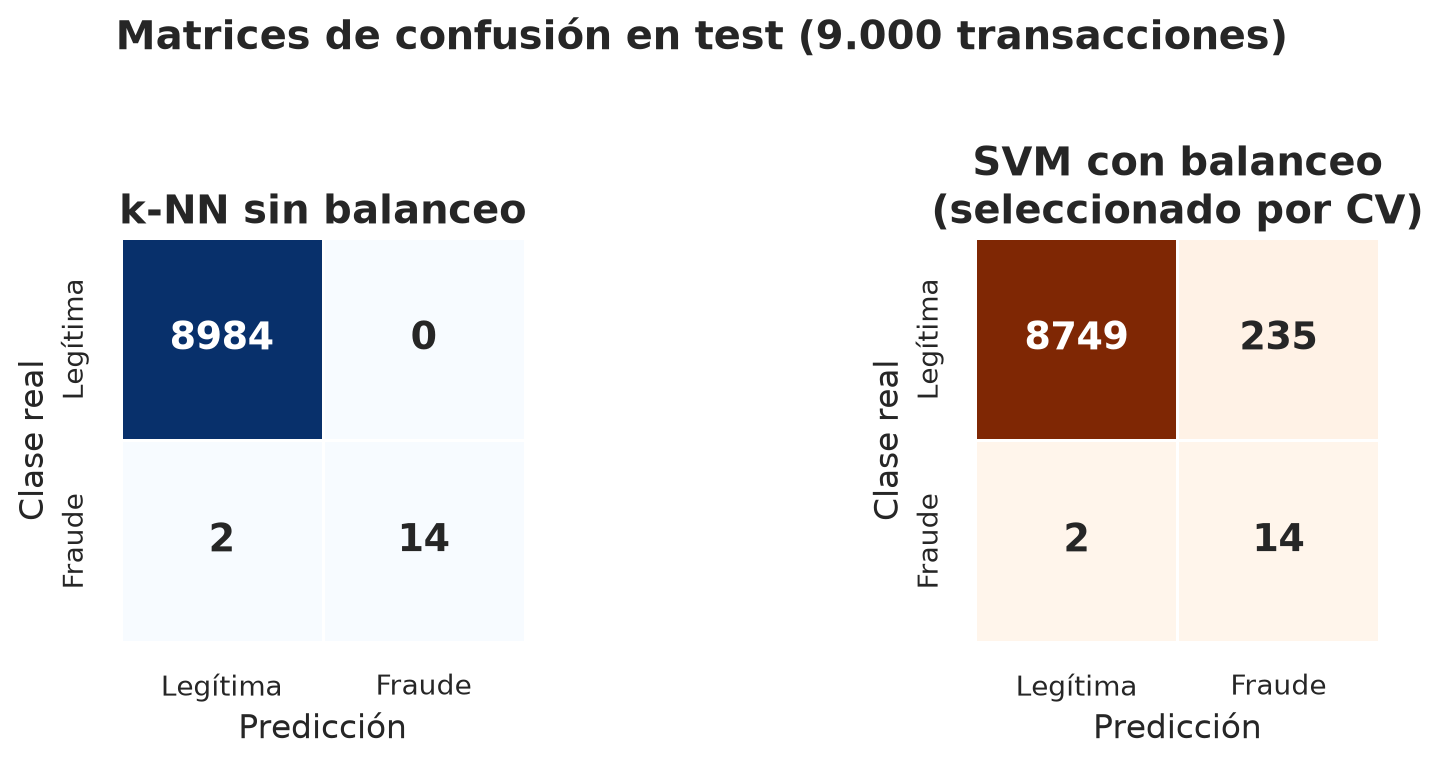
\includegraphics[width=\linewidth]{selected_confusions.png}
    \column{.44\textwidth}
      \small
      \begin{itemize}\setlength\itemsep{.45em}
        \item \textbf{Exactitud engañosa:} siempre legítima logra 99,82\%, pero
              sensibilidad 0 y FNR 1.
        \item \textbf{Compensar no ayuda igual a todos:} SVM sube en CV, pero en
              test conserva 14/16 fraudes y agrega 235 falsas alarmas.
        \item \textbf{Árbol vs. bosque:} con balanceo ambos detectan 12/16; el
              árbol produce 6 FP y el RF propio 0. Bagging mejora estabilidad en
              este test, sin garantía universal.
        \item \textbf{Siempre fraude:} FNR 0, pero 8.984 FP, precisión 0,18\% y
              exactitud 0,18\%: operacionalmente inviable.
      \end{itemize}
  \end{columns}
\end{frame}

% 11
\begin{frame}{10. Conclusiones y limitaciones}
  \small
  \begin{columns}[T,onlytextwidth]
    \column{.49\textwidth}
      \begin{block}{Qué aprendimos}
        \begin{itemize}\setlength\itemsep{.30em}
          \item CV seleccionó SVM lineal + \ros{} por sensibilidad 0,9179.
          \item En test detectó 14/16 fraudes, pero solo 5,62\% de sus alertas
                correspondieron a fraude.
          \item El RF propio demuestra bootstrap, diversidad de atributos y
                votación; con \ros{} obtuvo F1 0,8571 y cero FP en este test.
          \item La exactitud aislada no representa el objetivo del problema.
        \end{itemize}
      \end{block}
    \column{.49\textwidth}
      \begin{block}{Límites y próximos pasos}
        \begin{itemize}\setlength\itemsep{.30em}
          \item Solo 52 fraudes en la muestra y 16 en test: alta incertidumbre.
          \item Variables PCA sin semántica disponible; explicabilidad limitada.
          \item Sobremuestreo replica casos y puede favorecer sobreajuste.
          \item Evaluar el dataset completo, calibrar probabilidades y elegir
                umbral según costos de FN/FP.
          \item Validar temporalmente ante cambio de patrones de fraude.
        \end{itemize}
      \end{block}
  \end{columns}
  \vspace{.15em}
  \centering\normalsize\good{Decisión recomendada: priorizar sensibilidad, pero medir siempre el costo operativo.}
\end{frame}

\appendix

% Respaldo A
\begin{frame}{Respaldo A. Configuraciones seleccionadas por condición}
  \scriptsize
  \renewcommand{\arraystretch}{1.13}
  \begin{tabular}{llp{.58\textwidth}}
    \toprule
    Modelo & Condición & Mejor configuración por CV \\
    \midrule
    k-NN & sin \ros{} & \(k=11\), Manhattan, pesos por distancia \\
    k-NN & con \ros{} & \(k=5\), euclídea, pesos por distancia \\
    SVM & sin \ros{} & lineal, \(C=2\) \\
    SVM & con \ros{} & lineal, \(C=0{,}5\) \\
    Árbol & sin \ros{} & entropía, profundidad 12, split 20, hoja 5 \\
    Árbol & con \ros{} & gini, profundidad libre, split 20, hoja 5 \\
    RF propio & sin \ros{} & 11 árboles, profundidad libre, \texttt{max\_features=sqrt} \\
    RF propio & con \ros{} & 11 árboles, profundidad libre, \texttt{max\_features=sqrt} \\
    \bottomrule
  \end{tabular}
\end{frame}

% Respaldo B
\begin{frame}{Respaldo B. Métricas completas de validación cruzada}
  \centering
  \fontsize{5.6}{6.7}\selectfont
  \renewcommand{\arraystretch}{1.16}
  \begin{tabular}{llrrrrrr}
    \toprule
    Modelo & Cond. & Sensibilidad & Especificidad & Precisión & F1 & Exactitud & FNR \\
    \midrule
    k-NN & sin & .8321±.0593 & .9997±.0002 & .8281±.1029 & .8254±.0576 & .9994±.0002 & .1679±.0593 \\
    k-NN & con & .8321±.0593 & .9995±.0002 & .7590±.0816 & .7913±.0574 & .9992±.0002 & .1679±.0593 \\
    SVM & sin & .7464±.1692 & .9997±.0003 & .8614±.1240 & .7737±.0910 & .9993±.0002 & .2536±.1692 \\
    SVM & con & .9179±.0674 & .9713±.0116 & .0596±.0214 & .1109±.0368 & .9712±.0115 & .0821±.0674 \\
    Árbol & sin & .7250±.0746 & .9996±.0003 & .7679±.1354 & .7384±.0686 & .9991±.0003 & .2750±.0746 \\
    Árbol & con & .7786±.0655 & .9995±.0003 & .7367±.0921 & .7510±.0451 & .9991±.0003 & .2214±.0655 \\
    RF propio & sin & .6357±.1974 & .9998±.0003 & .9048±.1313 & .7136±.1467 & .9992±.0003 & .3643±.1974 \\
    RF propio & con & .7750±.1172 & .9998±.0003 & .8829±.1115 & .8105±.0507 & .9994±.0002 & .2250±.1172 \\
    \bottomrule
  \end{tabular}

  \vspace{.7em}
  \small Media ± desviación estándar poblacional entre cinco folds del 70\% de entrenamiento.
\end{frame}

% Respaldo C
\begin{frame}{Respaldo C. Métricas completas de prueba (1/2)}
  \centering
  \fontsize{6.2}{7.4}\selectfont
  \renewcommand{\arraystretch}{1.2}
  \begin{tabular}{llrrrrrr}
    \toprule
    Modelo & Cond. & Sensibilidad & Especificidad & Precisión & F1 & Exactitud & FNR \\
    \midrule
    k-NN & sin & .8750±.0852 & 1.0000±.0000 & 1.0000±.0000 & .9333±.0495 & .9998±.0002 & .1250±.0852 \\
    k-NN & con & .8750±.0852 & .9997±.0002 & .8235±.0805 & .8485±.0655 & .9994±.0002 & .1250±.0852 \\
    SVM & sin & .6875±.1226 & 1.0000±.0000 & 1.0000±.0000 & .8148±.0874 & .9994±.0002 & .3125±.1226 \\
    SVM & con & .8750±.0852 & .9738±.0017 & .0562±.0063 & .1057±.0117 & .9737±.0017 & .1250±.0852 \\
    \bottomrule
  \end{tabular}

  \vspace{1em}
  \small Punto estimado ± desviación bootstrap estratificada de 200 remuestras de
  las predicciones fijas. No son múltiples entrenamientos.
\end{frame}

% Respaldo D
\begin{frame}{Respaldo D. Métricas completas de prueba (2/2)}
  \centering
  \fontsize{6.2}{7.4}\selectfont
  \renewcommand{\arraystretch}{1.2}
  \begin{tabular}{llrrrrrr}
    \toprule
    Modelo & Cond. & Sensibilidad & Especificidad & Precisión & F1 & Exactitud & FNR \\
    \midrule
    Árbol & sin & .5000±.1187 & 1.0000±.0000 & 1.0000±.0000 & .6667±.1038 & .9991±.0002 & .5000±.1187 \\
    Árbol & con & .7500±.1077 & .9993±.0003 & .6667±.0952 & .7059±.0828 & .9989±.0003 & .2500±.1077 \\
    RF propio & sin & .6875±.1226 & 1.0000±.0000 & 1.0000±.0000 & .8148±.0874 & .9994±.0002 & .3125±.1226 \\
    RF propio & con & .7500±.1077 & 1.0000±.0000 & 1.0000±.0000 & .8571±.0719 & .9996±.0002 & .2500±.1077 \\
    \bottomrule
  \end{tabular}

  \vspace{1em}
  \small Punto estimado ± desviación bootstrap estratificada de 200 remuestras de
  las predicciones fijas. Matrices completas: \texttt{results/figures/issue\_8\_confusion\_matrices.png}.
\end{frame}

\end{document}
